\section{Performance Evaluation} \label{eval}

\subsection{Methodology}

\begin{figure*}[htb!]
\begin{minipage}[t]{0.45\textwidth}
\centerline{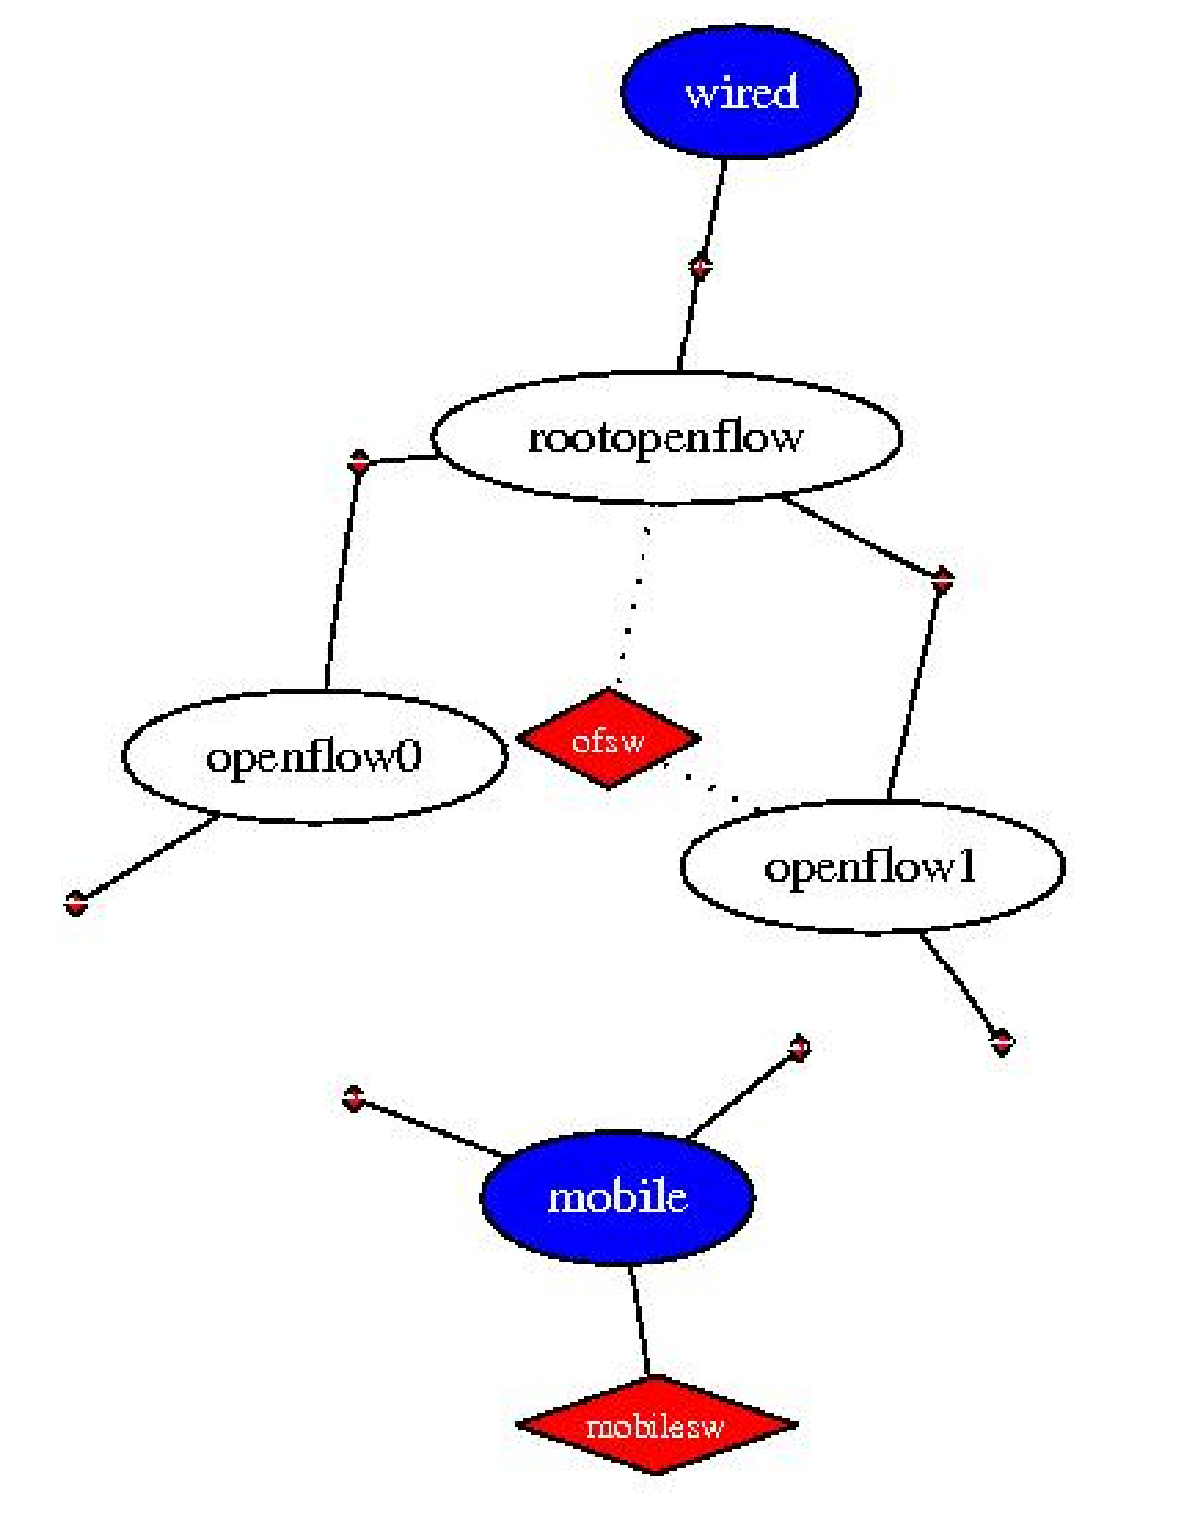
\includegraphics[width=\columnwidth]{fig/hoolock_handover}}
\caption{Simulation topology for evaluation of \sys{}.}
\label{fig:hoolock_topo}
\end{minipage}
\hfill
\begin{minipage}[t]{0.45\textwidth}
\centerline{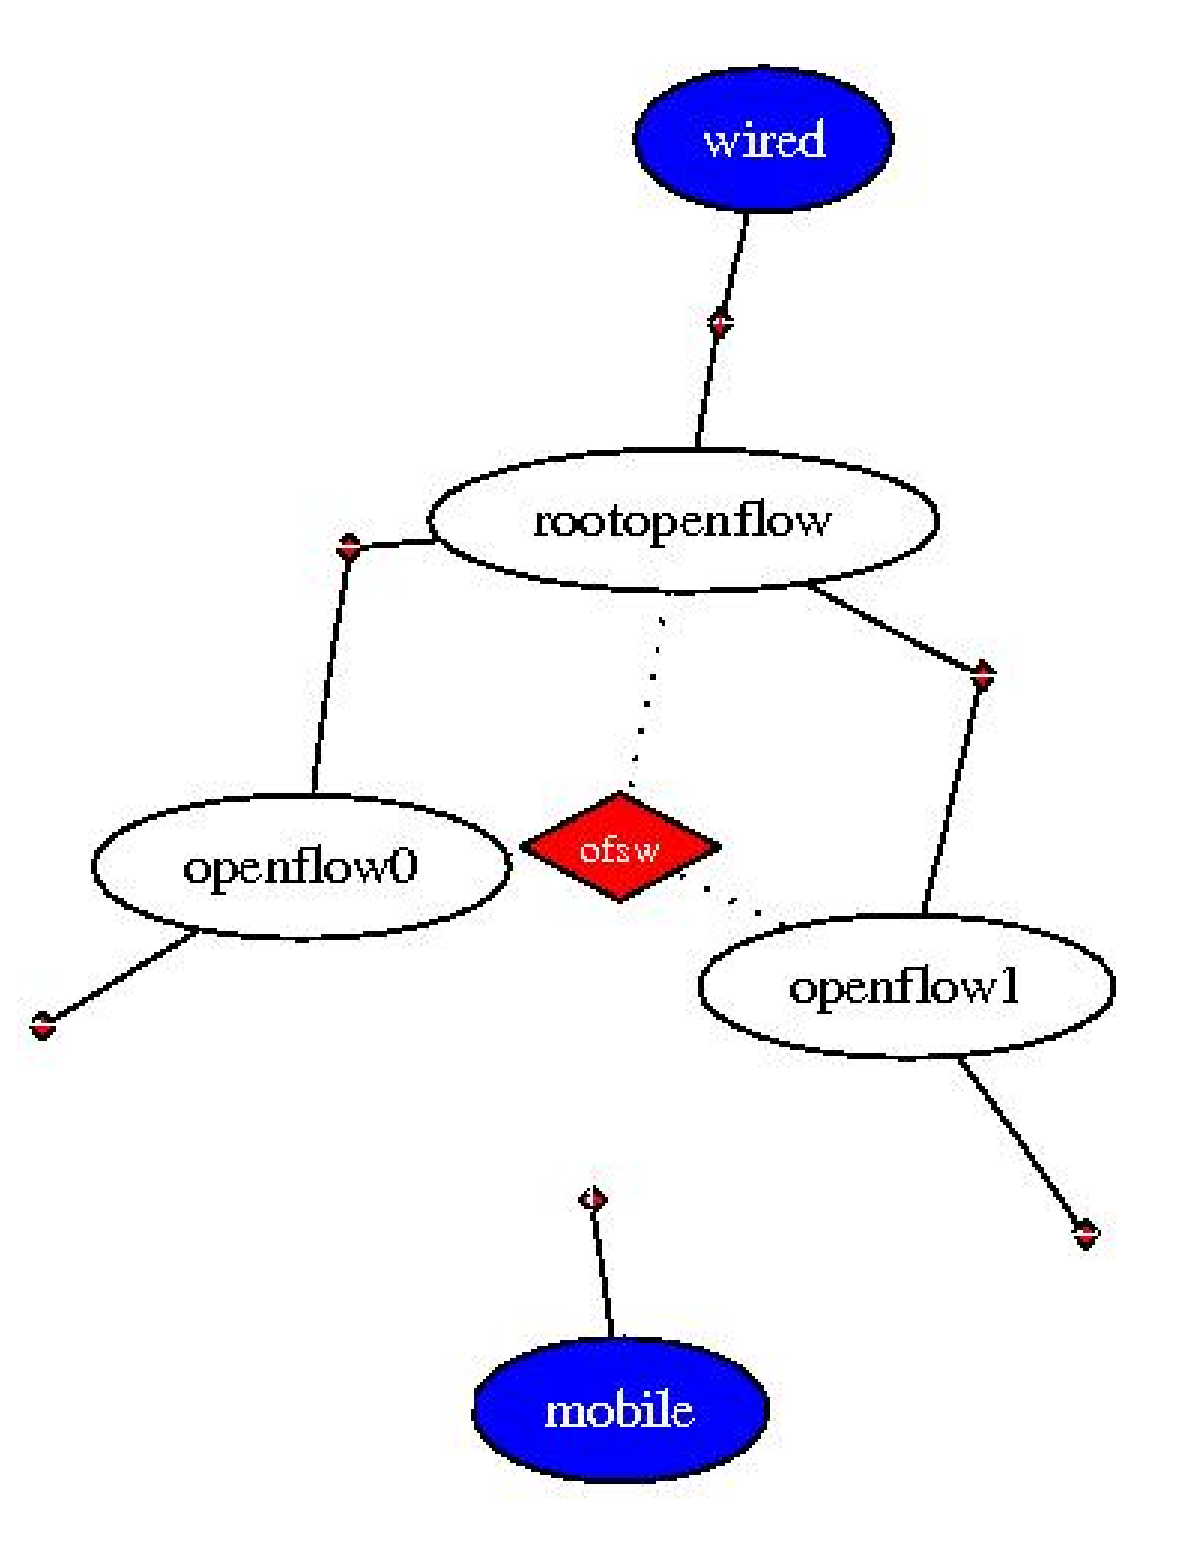
\includegraphics[width=\columnwidth]{fig/hard_handover}}
\caption{Simulation topology for evaluation of hard handoff.}
\label{fig:hard_topo}
\end{minipage}
\hfill
\end{figure*}

We use Virtual Distributed Ethernet (VDE) to evaluate the performance of \sys, 
and compare it with that of hard handoff and the base-case of no handoff.
We assume hard handoff requires approximately $150$ ms to scan the available 
channels before associating with a new AP.
Figures~\ref{fig:hoolock_topo} and~\ref{fig:hard_topo} show the topologies of 
the networks used in the simulation of \sys{} and hard-handoff respectively. 
The topology consists of three OpenFlow switches - $rootopenflow$, $openflow0$, and $openflow1$ 
and two clients - $wired$ and $mobile$.

We simulate the association and dissociation of $mobile$ with the OpenFlow switches by
creating and destroying pipes. We use wirefilter to simulate the link quality parameters
such as delay, loss, and loss-burst.

We evaluate the performance of various handoff schemes by transferring UDP data
from $wired$ to $mobile$ using iperf for $20$ seconds, and various rates, and initiating a 
handoff roughly half way through the transfer. We use the loss rate reported by
iperf as the performance metric.

\subsection{Results}

\begin{figure*}[htb!]
\begin{minipage}[t]{0.45\textwidth}
\centerline{\includegraphics[width=\columnwidth]{fig/lossless}}
\caption{Hard-handover packet loss in a lossless topology.}
\label{fig:lossless}
\end{minipage}
\hfill
\begin{minipage}[t]{0.45\textwidth}
\centerline{\includegraphics[width=\columnwidth]{fig/lossy}}
\caption{Packet loss in a lossy topology.}
\label{fig:lossy}
\end{minipage}
\hfill
\end{figure*}

\begin{figure*}[htb!]
\begin{minipage}[t]{0.45\textwidth}
\centerline{\includegraphics[width=\columnwidth]{fig/lossless_timeseries}}
\caption{Packet loss in a lossless topology.}
\label{fig:lossless_ts}
\end{minipage}
\hfill
\begin{minipage}[t]{0.45\textwidth}
\centerline{\includegraphics[width=\columnwidth]{fig/lossy_timeseries}}
\caption{Packet loss in a lossy topology.}
\label{fig:lossy_ts}
\end{minipage}
\hfill
\end{figure*}

Figure~\ref{fig:lossless} shows the number of packets lost during a hard handoff 
for various traffic rates in a lossless topology. 
We observe that the number of packets lost increases
with increasing traffic rate. This is due to the packets that get dropped during
the time period between the dissociation and association of $mobile$ with an AP.
The loss experienced by \sys{} was consistently zero. Hence, we do not plot those results.

Figure~\ref{fig:lossless_ts} shows a typical variation of packet loss during various 
$2$-second intervals with time. While \sys{} and no-handoff experience zero loss consistently,
hard-handoff experiences a large spike during the handoff period.

Figure~\ref{fig:lossy} shows the number of packets lost by various handoff 
schemes in a topology where the last-hop link has a loss rate of $10\%$ and a loss-burst
of $1.5$. 
We can observe that the loss experienced by \sys{} is statistically equivalent to that 
experienced when there is no handoff, which is due to the loss induced by lossy links.
On the other hand, hard-handoff experiences a much larger data loss.
This result can be better understood by the time-series graph in~\ref{fig:lossy_ts}, which 
shows that \sys{} performs as well as no-handoff, while hard-handoff experiences a spike
in packet loss during the handoff period.

Thus, \sys{} enables truly seamless mobility and provides data transfer equivalent to continuous transmission without handover.

